\documentclass[UTF8]{ctexart}
\usepackage{ctex}
\usepackage{geometry}
\usepackage{enumitem}
\usepackage{indentfirst}
\usepackage{color}
\usepackage{fancyhdr}
\usepackage{amsmath}
\usepackage{graphicx}
\usepackage{amssymb}
\usepackage{tikz}
\usepackage{cases}
\usepackage{array}
\usepackage{mathrsfs}

% 设置纸张和页边距——A4
\geometry{papersize={21cm,29.7cm}}
\geometry{left=3.18cm,right=3.18cm,top=2.54cm,bottom=2.54cm}

% 一级标题靠左
\CTEXsetup[format={\Large\bfseries}]{section}

% 去除页眉
\pagestyle{plain}

% 开始文档内容
\begin{document}

\title{信号与系统课程笔记:Lecture 13}
\author{授课教师:秦雨潇 \\
        笔记记录:李梦薇}
\date{2023 年 11 月 01 日(第九周,周三)}
\maketitle

\section{复习}
Fourier Transfrom $=\lim_{T\to+\infty}$ Fourier Series\par
$f(t)=\sum_{n=-\infty}^{+\infty}F[\omega]e^{j\omega{t}}\qquad\omega=n\Omega$,$t\in[-\frac{T}{2},\frac{T}{2}]$ \par
$F[\omega]=\frac{1}{T}\int_{0}^{T}f(t)e^{-j\omega{t}}{\rm{dt}}$ \par

\section{傅里叶变换(Fourier Transfrom,FT)}
\subsection{推导}
\noindent
\begin{flalign*}\hspace{2em}
    \lim_{T\to+\infty}f(t)&=\lim_{T\to+\infty}\sum_{n=-\infty}^{+\infty}F[\omega]e^{j\omega{t}} &\\
    &=\lim_{T\to+\infty}\sum_{n=-\infty}^{+\infty}\frac{1}{T}\int_{-\frac{T}{2}}^{\frac{T}{2}}f(\xi)e^{-j\omega\xi}{\rm{d\xi}}\cdot{e^{j\omega{t}}} &\\
    &=\int_{-\infty}^{+\infty}\frac{{\rm{d}}\omega}{2\pi}\int_{-\infty}^{+\infty}f(\xi)e^{-j\omega\xi}{\rm{d\xi}}\cdot{e^{j\omega{t}}} &\\
    &=\int_{-\infty}^{+\infty}\frac{1}{2\pi}\int_{-\infty}^{+\infty}f(\xi)e^{-j\omega\xi}{\rm{d\xi}}\cdot{e^{j\omega{t}}}{\rm{d}}\omega &\\
    &=\frac{1}{2\pi}\int_{-\infty}^{+\infty}F(\omega)e^{j\omega{t}}{\rm{d}}\omega
\end{flalign*} \par
因此,傅里叶变换公式为:\par
\noindent
\begin{flalign*}\hspace{2em}
    &F(\omega)=\int_{\mathbb{R}}f(t)e^{-j\omega{t}}{\rm{d}}t &\\
    &f(t)=\frac{1}{2\pi}\int_{\mathbb{R}}F(\omega)e^{j\omega{t}}{\rm{d}}\omega
\end{flalign*} \par
令$\omega=2\pi{f}$,傅里叶变换公式为:\par
\noindent
\begin{flalign*}\hspace{2em}
    &F(f)=\int_{\mathbb{R}}f(t)e^{-j2\pi{ft}}{\rm{d}}t &\\
    &f(t)=\frac{1}{2\pi}\int_{\mathbb{R}}F(f)e^{j2\pi{ft}}{\rm{d}}f
\end{flalign*} \par

\subsection{说明}
\begin{enumerate}[label=(\arabic*),itemindent=0pt,labelindent=\parindent,labelwidth=2em,labelsep=5pt,leftmargin=*]
    \item Continuous Time Fourier Transfrom(CTFT)
    \item “notation”:$F(j\omega)$,$F(\omega)$,$\hat{f}(\omega)$,$\mathscr{F}\{f(t)\}\qquad$
          注意:傅里叶逆变换写为$\mathscr{F}^{-1}\{f(t)\}$
\end{enumerate}\par

\subsection{性质}
\begin{enumerate}[label=(\arabic*),itemindent=0pt,labelindent=\parindent,labelwidth=2em,labelsep=5pt,leftmargin=*]
    \item Gibbs现象
          \begin{enumerate}[label=\textcircled{\arabic*}]
            \item “峰值”不会下降,大约是“高度”的9$\%$
            \item 随着累加,“波纹”的宽度会被进一步压缩,趋向于0
          \end{enumerate}
          \begin{figure}[h]
            \centering
            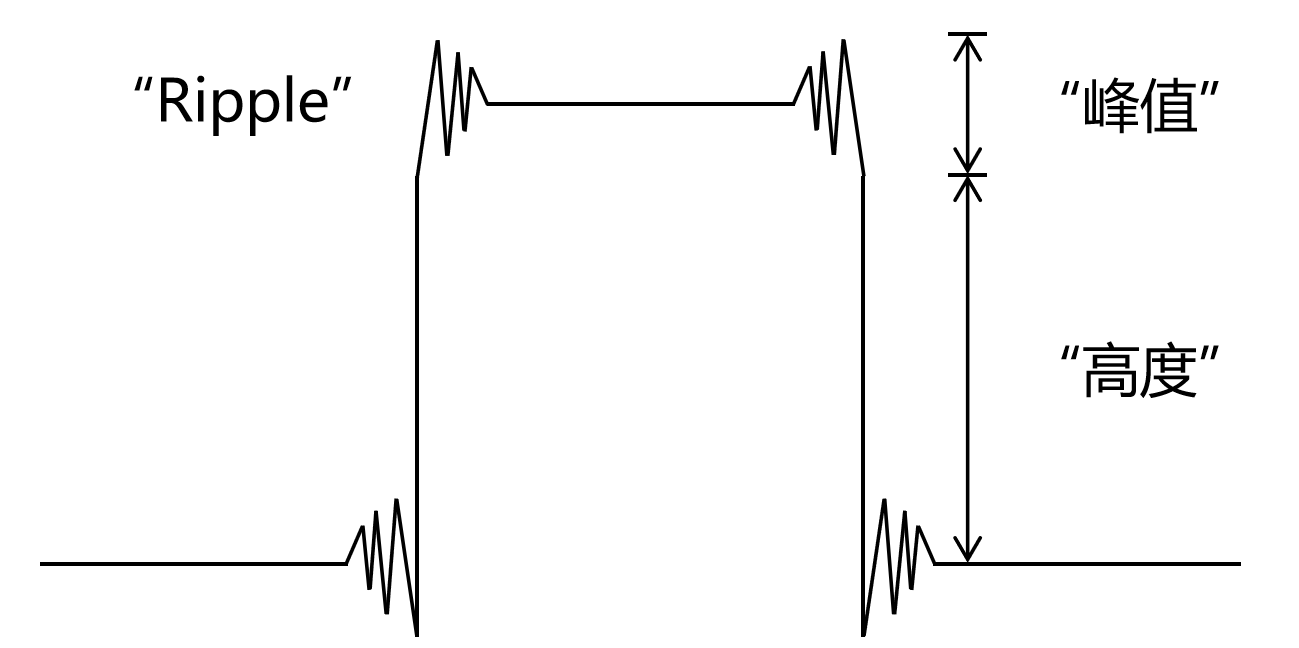
\includegraphics[scale=0.35]{Gibbs.png}
          \end{figure}
    \item Dirichlet条件(充分条件)
          \begin{enumerate}[label=\textcircled{\arabic*}]
            \item 绝对可积,$\int_{\mathbb{R}}|f(t)|{\rm{d}}t<+\infty$\par
                  证明:$|F(\omega)|\leqslant\int_{\mathbb{R}}|f(t)e^{-j\omega{t}}|{\rm{d}}t=\int_{\mathbb{R}}|f(t)|{\rm{d}}t<+\infty$
            \item 在任意区间$[a,b]$内,$f(t)$只有有限多个“第一类间断点”
            \item 在任意区间$[a,b]$内,$f(t)$只有有限多个极大值/极小值
          \end{enumerate}
\end{enumerate}\par

\subsection{例题}
\begin{enumerate}[label=(\arabic*),itemindent=0pt,labelindent=\parindent,labelwidth=2em,labelsep=5pt,leftmargin=*]
    \item $f(t)=e^{-\alpha{t}}U(t)$ \par
          \noindent
          \begin{flalign*}
            F(\omega)&=\int_{0}^{+\infty}e^{-\alpha{t}}e^{-j\omega{t}}{\rm{d}}t &\\
            &=\int_{0}^{+\infty}e^{-(\alpha+j\omega)t}{\rm{d}}t &\\
            &=\frac{1}{-(\alpha+j\omega)}e^{-(\alpha+j\omega)t}\big{|}_{0}^{+\infty} &\\
            &=\frac{1}{-(\alpha+j\omega)}(0-1) &\\
            &=\frac{1}{\alpha+j\omega}
          \end{flalign*}
    \item $f(t)=e^{-\alpha{|t|}}$ \par
          \noindent
          \begin{flalign*}
            F(\omega)&=\int_{0}^{+\infty}e^{-\alpha{t}}e^{-j\omega{t}}{\rm{d}}t+\int_{-\infty}^{0}e^{\alpha{t}}e^{-j\omega{t}}{\rm{d}}t &\\
            &=\frac{1}{\alpha+j\omega}+\frac{1}{\alpha-j\omega} &\\
            &=\frac{2\alpha}{\alpha^2+\omega^2}
          \end{flalign*}
    \item $g_{\tau}(t)=\left\{
          \begin{array}{cl}
          1 &  t\in[-\frac{\tau}{2},\frac{\tau}{2}] \\
          0 &  e.e. \\
          \end{array} \right.$ \par
          $F(\omega)=\tau{Sa(\frac{\omega{\tau}}{2})}$
    \item $\delta(t)$ \par
          $F(\omega)=\int_{\mathbb{R}}\delta(t)e^{-j\omega{0}}{\rm{d}}t=1$
\end{enumerate}\par

\subsection{特殊情况}
\noindent\textbf{问题:}\par
一系列不满足绝对可积的函数,如何进行傅里叶变换?\par
\noindent\textbf{思路(极限思维):}\par
如果可以构造$f(t)=\lim_{n\to+\infty}f_n(t)$,且$f_n(t)$满足Dirichlet条件,则$F(\omega)=\lim_{n\to+\infty}F_n(\omega)$统称为广义傅里叶变换。\par
\noindent\textbf{举例:}\par
$\mathscr{F}\{f(t)\}$,其中$f(t)=1$,如何进行傅里叶变换?\par
\begin{enumerate}[label=(\arabic*),itemindent=0pt,labelindent=\parindent,labelwidth=2em,labelsep=5pt,leftmargin=*]
  \item $e^{-\alpha{|t|}}\rightleftharpoons\frac{2\alpha}{\alpha^2+\omega^2}$ \par
        $\alpha\rightarrow0\qquad e^{-\alpha{|t|}}\rightarrow1$ \par
        $\mathscr{F}\{f(t)=1\}=\lim_{\alpha\to0}\mathscr{F}\{e^{-\alpha{|t|}}\}
        =\lim_{\alpha\to0}\frac{2\alpha}{\alpha^2+\omega^2}=\left\{
        \begin{array}{cl}
          +\infty &  \omega=0 \\
          0 &  \omega\neq0 \\
        \end{array} \right. $ \par
        $\int_{\mathbb{R}}\lim_{\alpha\to0}\frac{2\alpha}{\alpha^2+\omega^2}{\rm{d}}\omega
        =\lim_{\alpha\to0}\int_{\mathbb{R}}\frac{2\alpha}{\alpha^2+\omega^2}{\rm{d}}\omega
        =2\arctan(\frac{\omega}{\alpha})\big{|}_{-\infty}^{+\infty}=2\pi$ \par
        则$1\rightleftharpoons2\pi\delta(t)$
  \item $\lim_{\tau\to0}Sa(\frac{\omega\tau}{2})=\left\{
        \begin{array}{cl}
          +\infty &  t=0 \\
          0 &  t\neq0 \\
        \end{array} \right. $ \par
\end{enumerate}\par

\section{傅里叶变换的性质}
\begin{enumerate}[label=(\arabic*),itemindent=0pt,labelindent=\parindent,labelwidth=2em,labelsep=5pt,leftmargin=*]
    \item \textbf{线性:}if $f_1(t)\rightleftharpoons{F_1(\omega)}$,$f_2(t)\rightleftharpoons{F_2(\omega)}$ \par
          \begin{itemize}[label=,left=2.5em]
            \item than $af_1(t)+bf_2(t)\rightleftharpoons{aF_1(\omega)}+bF_2(\omega)$
          \end{itemize}
    \item 奇偶性:if $f(t)\rightleftharpoons{F(\omega)}$ \par
          \begin{itemize}[label=,left=3.5em]
            \item than $f(-t)\rightleftharpoons{F(-\omega)}$
          \end{itemize}
    \item 对称性:if $f(t)\rightleftharpoons{F(\omega)}$ \par
          \begin{itemize}[label=,left=3.5em]
            \item than $F(t)\rightleftharpoons2\pi{f(-\omega)}$
          \end{itemize}
    \item \textbf{尺度变换:}if $f(t)\rightleftharpoons{F(\omega)}$ \par
          \begin{itemize}[label=,left=4.5em]
            \item than $f(\alpha{t})\rightleftharpoons\frac{1}{|\alpha|}{F(\frac{\omega}{\alpha})}$
          \end{itemize}
    \item 频移/时移:if $f(t)\rightleftharpoons{F(\omega)}$ \par
          时移:$f(t\pm{t_0})\rightleftharpoons{e^{\pm{j\omega{t_0}}}F(\omega)}$ \par
          频移:$f(t)e^{\mp{j\omega_0t}}\rightleftharpoons{F(\omega\pm\omega_0)}$ \par
    \item \textbf{卷积定理:}if $f_1(t)\rightleftharpoons{F_1(\omega)}$,$f_2(t)\rightleftharpoons{F_2(\omega)}$ \par
          \begin{itemize}[label=,left=4.5em]
            \item than $f_1(t)*f_2(t)\rightleftharpoons{F_1(\omega)F_2(\omega)}$
          \end{itemize} \par
          证明:$\int_{\mathbb{R}}[f_1(\tau)f_2(t-\tau){\rm{d}}\tau]\cdot{e^{-j\omega{t}}}{\rm{d}}t$
          \begin{itemize}[label=,left=2.5em]
            \item $=\int_{\mathbb{R}}f_1(\tau){\rm{d}}\tau\int_{\mathbb{R}}f_2(t-\tau)\cdot{e^{-j\omega(t-\tau)}}{\rm{d}}(t-\tau)\cdot{e^{-j\omega{\tau}}}$
            \item $=\int_{\mathbb{R}}f_1(\tau){\rm{d}}\tau\int_{\mathbb{R}}f_2(\xi)\cdot{e^{-j\omega(\xi)}}{\rm{d}}(\xi)\cdot{e^{-j\omega{\tau}}}$
            \item $=\int_{\mathbb{R}}f_1(\tau){e^{-j\omega{\tau}}}{\rm{d}}\tau\cdot{F_2(\omega)}$
            \item $=F_1(\omega)F_2(\omega)$
          \end{itemize} \par
    \item Parseval's定理:if $f(t)\rightleftharpoons{F(\omega)}$ \par
          \begin{itemize}[label=,left=7.1em]
            \item than $\int_{\mathbb{R}}|f(t)|^2{\rm{d}}t=\frac{1}{2\pi}\int_{\mathbb{R}}|F(\omega)|^2{\rm{d}}\omega$
          \end{itemize}
    \item 时域/频域,微分/积分(自己看书学习!)
\end{enumerate}\par

\end{document}